%!TEX root = ../DA_MainDocument.tex

% ============================================================
\chapter{Implementierung: Benachrichtigungs- und Erinnerungsmodul (JanOle)}
\label{chapter:notifications}
% ============================================================

Dieses Kapitel beschreibt die technische Umsetzung des Benachrichtigungs- und
Erinnerungsmoduls in Skyline.
Die konzeptionellen Grundlagen -- proaktive Assistenz, Unterbrechungskosten, Notification
Fatigue sowie Anforderungen im Reise-Kontext -- wurden in Kapitel~3 erarbeitet.
Die hier gezeigte Implementierung setzt diese Anforderungen als mehrstufiges Reminder-System
um und kombiniert lokales Scheduling auf dem Endgerät mit einer serverseitigen Registry,
um Nachvollziehbarkeit und Robustheit zu erhöhen
\cite{ozdemir2025echoes,visuri2019notifications}.

Skyline wurde primär für \textbf{iOS} entwickelt und ist im \textbf{Apple App Store}
verfügbar \cite{appleLocalNotif}.
Die Zielplattform der gesamten Implementierung -- inklusive des Benachrichtigungsmoduls --
ist damit iOS mit dem Apple Push Notification Service (APNs) als Plattformgrundlage.
Eine Android-Kompatibilitätsschicht ist im Code vorhanden, wurde jedoch nicht vollständig
getestet und gilt als nachrangig.

Ziel des Moduls ist es, typische Stress- und Fehlerfälle vor und nach Flügen zu reduzieren
(z.\,B. verpasster Check-in, fehlende Unterlagen, vergessene Belege), ohne Nutzerinnen und
Nutzer durch zu häufige oder irrelevante Benachrichtigungen zu überlasten.
Technisch wird dies durch feste Reminder-Offsets, konfigurierbare Settings, eine
Quiet-Hours-Logik sowie Deep-Links in die passende App-Ansicht erreicht
\cite{ozdemir2025echoes,reactNavDeepLink}.

% ============================================================
\section{Implementierung in Skyline}
\label{sec:notifications-implementation}
% ============================================================

Die Implementierung des Reminder-Moduls basiert auf zwei Säulen:

\begin{itemize}
  \item \textbf{Lokale Benachrichtigungen} über \texttt{expo-notifications}, inklusive
        Scheduling, Cancel und Handling von Nutzer-Interaktionen
        \cite{expoNotificationsSDK,expoHandleIncoming}.
  \item \textbf{Serverseitige Reminder-Registry} in Supabase (Tabelle \texttt{notifications}),
        um geplante Erinnerungen zu persistieren, nach App-Neustart erneut einplanen zu
        können und den Status (z.\,B. \texttt{pending}/\texttt{scheduled\_local}/
        \texttt{cancelled}/\texttt{failed}) nachvollziehbar zu halten
        \cite{supabaseRLS,supabaseSecuringApi}.
\end{itemize}

Die App kapselt Benachrichtigungslogik in einer Service-Schicht,
um UI und Scheduling klar zu trennen. Zentrale Bausteine sind:

\begin{itemize}
  \item \texttt{services/notifications.ts} -- Abstraktion über \texttt{expo-notifications}
        inkl.\ Permission-Handling (iOS/APNs als Primärplattform), Quiet-Hours-Logik
        sowie einer Android-Channel-Schicht für zukünftige Kompatibilität
        \cite{expoNotificationsSDK,appleLocalNotif}.
  \item \texttt{services/flightAutoReminderService.ts} -- automatische Flight-Reminder
        (Check-in, Boarding, Missing Docs, Receipt).
  \item \texttt{services/noteChecklistReminderService.ts} -- Reminder für manuell gesetzte
        Notizen und Checklisten.
  \item \texttt{services/notificationRegistry.ts} -- Persistieren und Abfragen der Registry
        in Supabase \cite{supabaseSecuringApi}.
  \item \texttt{services/notificationRescheduler.ts} -- Re-Scheduling ausstehender Reminder
        nach App-Neustart oder Permission-Änderungen.
\end{itemize}

Die Initialisierung erfolgt beim App-Start.
Im Root-Layout (\texttt{app/\_layout.tsx}) wird nach erfolgreicher Authentifizierung
\texttt{initializeNotifications} aufgerufen.
Auf iOS werden dabei die Notification-Berechtigungen geprüft und -- sofern in den
Einstellungen vorgesehen -- über den systemseitigen Permission-Dialog von iOS angefragt
\cite{expoNotificationsSDK,appleLocalNotif}.
Zusätzlich werden Android-Notification-Channels angelegt; da Skyline primär für iOS
entwickelt und dort produktiv betrieben wird (\textbf{App Store}), sind diese Channels
als Kompatibilitätsvorbereitung zu verstehen und wurden auf Android nicht vollständig getestet
\cite{androidNotifChannels}.
Listing~\ref{lst:init_notif} zeigt die vollständige Initialisierungsfunktion:

\begin{lstlisting}[style=skyline-ts,
  caption={Vollstaendige Initialisierung: Permission-Check und Channel-Anlage
           (services/notifications.ts)},
  label={lst:init_notif}]
export const initializeNotifications = async (
  options?: { requestPermission?: boolean }
): Promise<NotificationInitResult> => {
  const Notifications = await loadNotificationsModule();
  if (!Notifications) {
    return {
      available: false,
      granted: false,
      status: 'unavailable',
      canAskAgain: false,
    };
  }

  const permission = await ensurePermissionGranted(
    Notifications,
    options?.requestPermission !== false
  );

  // Android-Channels anlegen (iOS ignoriert diese, da iOS keine
  // Channels kennt -- auf iOS gilt APNs-Permission als ausreichend):
  await Promise.allSettled([
    ensureReminderChannel(Notifications,
      { channelId: 'reminders',           channelName: 'Reminders' }),
    ensureReminderChannel(Notifications,
      { channelId: 'note-reminders',      channelName: 'Note Reminders' }),
    ensureReminderChannel(Notifications,
      { channelId: 'checklist-reminders', channelName: 'Checklist Reminders' }),
  ]);

  return {
    available: true,
    granted: permission.granted,
    status: permission.status,
    canAskAgain: permission.canAskAgain,
  };
};
\end{lstlisting}

Abbildung~\ref{fig:reminder-architecture} gibt einen Überblick über die Gesamtarchitektur.

\begin{figure}[htbp]
  \centering
  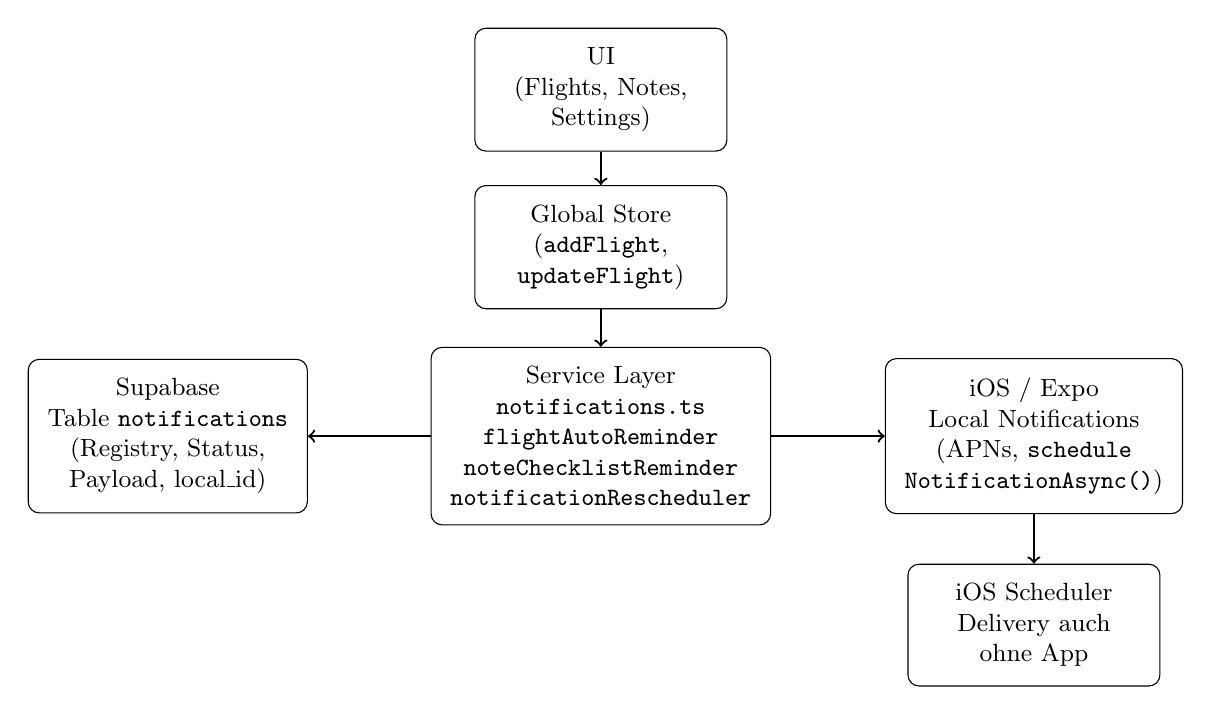
\begin{tikzpicture}[
    box/.style={draw, rounded corners, align=center, inner sep=7pt,
                minimum width=3.2cm, font=\small},
    arr/.style={->, thick}
  ]
    \node[box] (ui)      at (0, 0)    {UI\\(Flights, Notes,\\Settings)};
    \node[box] (store)   at (0,-2.0)  {Global Store\\(\texttt{addFlight},\\
                                       \texttt{updateFlight})};
    \node[box] (svc)     at (0,-4.4)  {Service Layer\\
                                       \texttt{notifications.ts}\\
                                       \texttt{flightAutoReminder}\\
                                       \texttt{noteChecklistReminder}\\
                                       \texttt{notificationRescheduler}};
    \node[box] (expo)    at (5.5,-4.4){iOS / Expo\\Local Notifications\\
                                       (APNs, \texttt{schedule}\\
                                       \texttt{NotificationAsync()})};
    \node[box] (os)      at (5.5,-6.8){iOS Scheduler\\Delivery auch\\ohne App};
    \node[box] (db)      at (-5.5,-4.4){Supabase\\Table \texttt{notifications}\\
                                       (Registry, Status,\\Payload, local\_id)};

    \draw[arr] (ui)    -- (store);
    \draw[arr] (store) -- (svc);
    \draw[arr] (svc)   -- (expo);
    \draw[arr] (svc)   -- (db);
    \draw[arr] (expo)  -- (os);
  \end{tikzpicture}
  \caption{Architektur des Reminder-Moduls: lokale Notifications plus serverseitige Registry}
  \label{fig:reminder-architecture}
\end{figure}

% ============================================================
\subsection{Reminder-Offsets und Scheduling-Flow}
\label{subsec:offsets-flow}
% ============================================================

Kern der Architektur ist die Definition fester Offsets relativ zu Abflug- und Ankunftszeit.
Tabelle~\ref{tab:reminder-offsets} fasst die Standard-Offsets zusammen.

\begin{table}[htbp]
  \centering
  \caption{Reminder-Typen und Default-Offsets in Skyline}
  \label{tab:reminder-offsets}
  \begin{tabularx}{\textwidth}{l l X}
    \toprule
    \textbf{Reminder-Typ} & \textbf{Offset} & \textbf{Motivation} \\
    \midrule
    Check-in     & T$-$24\,h            & Online-Check-in typischerweise im Vorfeldfenster
                                          \cite{lufthansaCheckin,lufthansaAutoCheckin} \\
    Boarding     & T$-$60\,min / T$-$30\,min & Boarding beginnt je nach Airline 60--25 bzw.\
                                          30--50\,min vor Abflug \cite{klmBoarding,aaBoarding} \\
    Missing Docs & T$-$12\,h            & Zeitpuffer für fehlende Unterlagen \\
    Receipt      & T$+$2\,h             & Belege für Reisekosten zeitnah erfassen
                                          \cite{mitSavingReceipts} \\
    \bottomrule
  \end{tabularx}
\end{table}

Abbildung~\ref{fig:reminder-timeline} visualisiert die Offsets auf einer Zeitachse.

\begin{figure}[htbp]
  \centering
  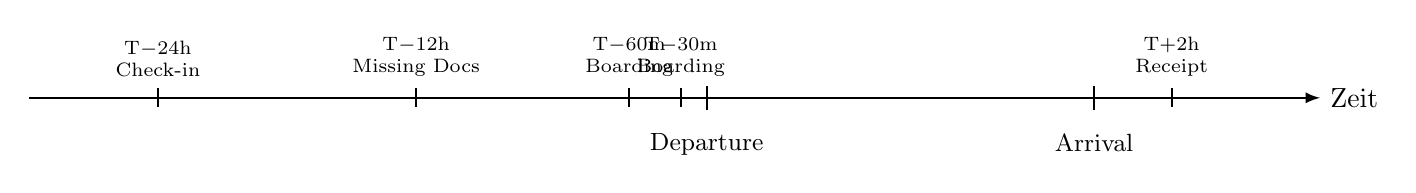
\begin{tikzpicture}[x=0.82cm, y=1cm, >=latex]
    \draw[->, thick] (-10.5,0) -- (9.5,0) node[right] {Zeit};

    \draw[thick] (0, 0.15) -- (0,-0.15) node[below=5pt] {\small Departure};
    \draw[thick] (6, 0.15) -- (6,-0.15) node[below=5pt] {\small Arrival};

    \draw[thick] (-8.5,0.12) -- (-8.5,-0.12);
    \node[above, align=center, font=\scriptsize] at (-8.5,0.15)
      {T$-$24h\\Check-in};

    \draw[thick] (-4.5,0.12) -- (-4.5,-0.12);
    \node[above, align=center, font=\scriptsize] at (-4.5,0.15)
      {T$-$12h\\Missing Docs};

    \draw[thick] (-1.2,0.12) -- (-1.2,-0.12);
    \node[above, align=center, font=\scriptsize] at (-1.2,0.15)
      {T$-$60m\\Boarding};

    \draw[thick] (-0.4,0.12) -- (-0.4,-0.12);
    \node[above, align=center, font=\scriptsize] at (-0.4,0.15)
      {T$-$30m\\Boarding};

    \draw[thick] (7.2,0.12) -- (7.2,-0.12);
    \node[above, align=center, font=\scriptsize] at (7.2,0.15)
      {T$+$2h\\Receipt};
  \end{tikzpicture}
  \caption{Standard-Offsets der Skyline-Reminder relativ zu Abflug und Ankunft}
  \label{fig:reminder-timeline}
\end{figure}

Die Berechnung der Trigger-Zeitpunkte erfolgt in \texttt{flightAutoReminderService.ts}.
Listing~\ref{lst:flight_offsets} zeigt die vollständige Funktion mit allen vier
Reminder-Typen:

\begin{lstlisting}[style=skyline-ts,
  caption={Vollstaendige scheduleAutoRemindersForFlight mit allen Offsets
           (services/flightAutoReminderService.ts)},
  label={lst:flight_offsets}]
export async function scheduleAutoRemindersForFlight(
  userId: string, flight: Flight
): Promise<void> {
  // Idempotent: bestehende Reminder zuerst loeschen
  await cancelAutoRemindersForFlight(userId, flight.id);

  const SettingsService = (await import('./settingsService')).default;
  const settings = await SettingsService.getInstance().getSettings();
  if (!settings.notifications) return;

  const { scheduleNotificationPersisted } = await import('./notifications');
  const ids: FlightReminderIds = {};

  const dep = flight.departureAt;
  const arr = flight.arrivalAt;
  if (!dep) return; // kein departureAt -> keine Reminder

  const urlTrip = `/trip-details?id=${flight.id}`;
  const urlDocs = `/trip-details?id=${flight.id}&tutorial=1`;

  // T-24h: Check-in-Reminder
  if (settings.reminderCheckIn) {
    const when = isoMinus(dep, 24 * 60 * 60 * 1000);
    const id = when
      ? await scheduleNotificationPersisted({
          userId,
          kind: 'flight.checkin',
          whenISO: when,
          title: 'Check-in available',
          body: 'Check-in is usually available 24h before departure.'
            + ' Open Trip Details to add/update info.',
          data: { url: urlTrip, flightId: flight.id },
        })
      : null;
    if (id) ids.checkin_24h = id;
  }

  // T-60min: erstes Boarding-Reminder
  if (settings.reminderBoarding) {
    const when60 = isoMinus(dep, 60 * 60 * 1000);
    const id60 = when60
      ? await scheduleNotificationPersisted({
          userId,
          kind: 'flight.boarding60',
          whenISO: when60,
          title: 'Boarding soon (flight)',
          body: 'Your flight boards in about 60 minutes.'
            + ' Check gate/terminal and make sure your docs are ready.',
          data: { url: urlDocs, flightId: flight.id },
        })
      : null;
    if (id60) ids.boarding_60m = id60;

    // T-30min: zweites Boarding-Reminder
    const when30 = isoMinus(dep, 30 * 60 * 1000);
    const id30 = when30
      ? await scheduleNotificationPersisted({
          userId,
          kind: 'flight.boarding30',
          whenISO: when30,
          title: 'Boarding soon (flight)',
          body: 'Your flight boards soon.'
            + ' Open Trip Details to check gate and documents.',
          data: { url: urlDocs, flightId: flight.id },
        })
      : null;
    if (id30) ids.boarding_30m = id30;
  }

  // T-12h: Missing-Docs-Reminder
  if (settings.reminderMissingDocs) {
    const when = isoMinus(dep, 12 * 60 * 60 * 1000);
    const id = when
      ? await scheduleNotificationPersisted({
          userId,
          kind: 'flight.missing_docs',
          whenISO: when,
          title: 'Documents check',
          body: 'Quick check: do you have your boarding pass'
            + ' / booking confirmation saved?'
            + ' Upload it now to avoid stress.',
          data: { url: urlDocs, flightId: flight.id },
        })
      : null;
    if (id) ids.missing_docs_12h = id;
  }

  // T+2h: Receipt-Reminder (nur wenn arrivalAt vorhanden)
  if (settings.reminderReceipt && arr) {
    const when = isoPlus(arr, 2 * 60 * 60 * 1000);
    const id = when
      ? await scheduleNotificationPersisted({
          userId,
          kind: 'flight.receipt',
          whenISO: when,
          title: 'Add receipts',
          body: "Don't forget to upload receipts"
            + ' for your business trip (hotel, taxi, etc.).',
          data: { url: urlDocs, flightId: flight.id },
        })
      : null;
    if (id) ids.receipt_2h = id;
  }

  // Alle vergebenen Notification-IDs in AsyncStorage sichern
  const store = await loadStore(userId);
  store[flight.id] = ids;
  await saveStore(userId, store);
}
\end{lstlisting}

% ============================================================
\subsection{Integration beim Flight-Save}
\label{subsec:flight-save}
% ============================================================

Damit das Reminder-Modul automatisch wirksam wird, ist es direkt im zentralen
Flight-Speicherpfad integriert.
Nach erfolgreichem Speichern eines Flugs in Supabase ruft der globale Store
(\texttt{store/index.ts}) im Hintergrund \texttt{scheduleAutoRemindersForFlight} auf.
Listing~\ref{lst:store_addflight} zeigt den relevanten Ausschnitt aus \texttt{addFlight}:

\begin{lstlisting}[style=skyline-ts,
  caption={Integration der Reminder-Logik beim Flight-Save (store/index.ts)},
  label={lst:store_addflight}]
// addFlight (store/index.ts) -- nach erfolgreichem Supabase-Insert:

// 1. Lokale Flight-Liste aktualisieren
set((state) => ({
  flights: [...state.flights, newFlight],
  isLoading: false,
}));
get().updateStats();

// 2. Auto-Reminder asynchron planen (blockiert nicht die UI)
try {
  const { scheduleAutoRemindersForFlight } = await import(
    '../services/flightAutoReminderService'
  );
  await scheduleAutoRemindersForFlight(user.id, newFlight);
} catch {}
\end{lstlisting}

Beim Update entscheidet der Store anhand des neuen Flugstatus, ob Reminder
gecancelt oder neu geplant werden:

\begin{lstlisting}[style=skyline-ts,
  caption={Reminder-Neuplanung bei Flug-Update (store/index.ts)},
  label={lst:store_updateflight}]
// updateFlight (store/index.ts) -- nach erfolgreichem Supabase-Update:
try {
  const user = get().user;
  if (user) {
    const {
      scheduleAutoRemindersForFlight,
      cancelAutoRemindersForFlight,
    } = await import('../services/flightAutoReminderService');

    if (
      normalizedFlight.status === 'cancelled' ||
      normalizedFlight.status === 'completed'
    ) {
      // Abgeschlossene/stornierte Fluege erhalten keine neuen Reminder
      await cancelAutoRemindersForFlight(user.id, normalizedFlight.id);
    } else {
      // Aktiver Flug: alte Reminder loeschen, neue auf Basis
      // der geaenderten Zeitdaten planen
      await scheduleAutoRemindersForFlight(user.id, normalizedFlight);
    }
  }
} catch {}
\end{lstlisting}

Beim Loeschen eines Flugs werden ebenfalls alle zugehoerigen Reminder entfernt:

\begin{lstlisting}[style=skyline-ts,
  caption={Reminder-Cancel beim Loeschen eines Flugs (store/index.ts)},
  label={lst:store_deleteflight}]
// deleteFlight (store/index.ts) -- nach erfolgreichem Supabase-Delete:
try {
  const user = get().user;
  if (user) {
    const { cancelAutoRemindersForFlight } = await import(
      '../services/flightAutoReminderService'
    );
    await cancelAutoRemindersForFlight(user.id, id);
  }
} catch {}
\end{lstlisting}

Abbildung~\ref{fig:sequence-flight-save} visualisiert den Ablauf als Sequenzdiagramm.

\begin{figure}[htbp]
  \centering
  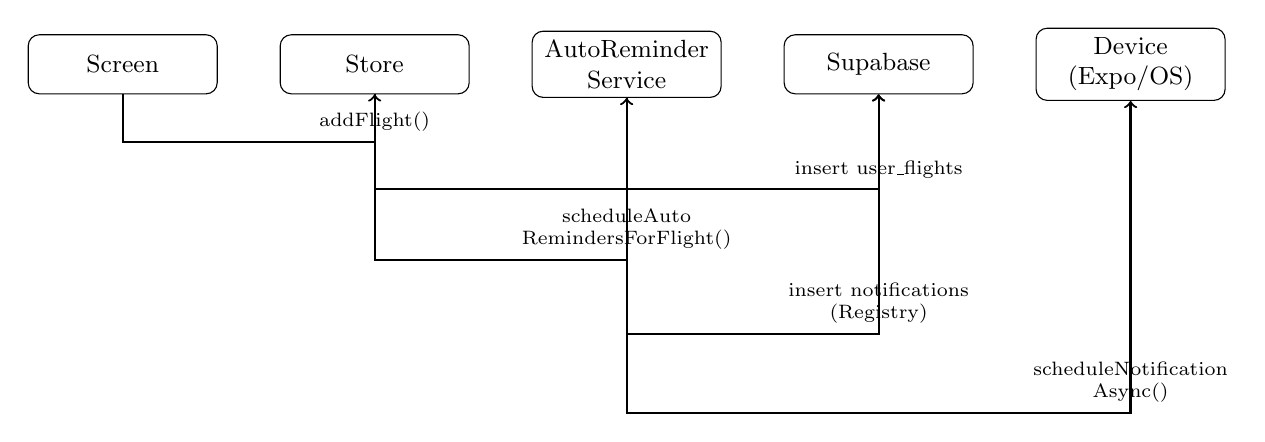
\begin{tikzpicture}[
    lifeline/.style={draw, rounded corners, align=center, minimum width=2.4cm,
                     minimum height=0.75cm, font=\small},
    arr/.style={->, thick},
    note/.style={font=\scriptsize, align=center}
  ]
    \node[lifeline] (screen) at (0,0)    {Screen};
    \node[lifeline] (store)  at (3.2,0)  {Store};
    \node[lifeline] (svc)    at (6.4,0)  {AutoReminder\\Service};
    \node[lifeline] (db)     at (9.6,0)  {Supabase};
    \node[lifeline] (dev)    at (12.8,0) {Device\\(Expo/OS)};

    \draw[arr] (screen.south) -- ++(0,-0.6) -| (store.south)
      node[midway, above, note] {addFlight()};
    \draw[arr] (store.south)  -- ++(0,-1.2) -| (db.south)
      node[midway, above, note] {insert user\_flights};
    \draw[arr] (store.south)  -- ++(0,-2.1) -| (svc.south)
      node[midway, above, note] {scheduleAuto\\RemindersForFlight()};
    \draw[arr] (svc.south)    -- ++(0,-3.0) -| (db.south)
      node[midway, above, note] {insert notifications\\(Registry)};
    \draw[arr] (svc.south)    -- ++(0,-4.0) -| (dev.south)
      node[midway, above, note] {scheduleNotification\\Async()};
  \end{tikzpicture}
  \caption{Sequenz beim Flight-Save: Store triggert Auto-Reminder, Registry und lokale Planung}
  \label{fig:sequence-flight-save}
\end{figure}

% ============================================================
\subsection{Quiet Hours}
\label{subsec:quiet-hours}
% ============================================================

Benachrichtigungen in Ruhezeiten werden von Forschung wiederholt als störend und
stressauslösend bewertet \cite{ozdemir2025echoes,visuri2019notifications}.
Skyline implementiert daher eine Quiet-Hours-Logik direkt in \texttt{notifications.ts}.
Liegt ein geplanter Reminder innerhalb des konfigurierten Ruhezeitfensters, wird er
automatisch auf das Ende des Fensters verschoben (\emph{bump}).
Listing~\ref{lst:quiet_hours} zeigt die vollständige Implementierung:

\begin{lstlisting}[style=skyline-ts,
  caption={Vollstaendige Quiet-Hours-Logik: isInQuietHours, bumpOutOfQuietHours
           und resolveScheduleTime (services/notifications.ts)},
  label={lst:quiet_hours}]
const isInQuietHours = (
  d: Date, startHHMM: string, endHHMM: string
): boolean => {
  const start = parseHHMM(startHHMM);
  const end   = parseHHMM(endHHMM);
  if (!start || !end) return false;
  const mins   = d.getHours() * 60 + d.getMinutes();
  const startM = start.h * 60 + start.m;
  const endM   = end.h   * 60 + end.m;
  if (startM === endM) return false;
  // Overnight-Fenster (z. B. 22:00 -> 07:00)
  if (startM > endM) return mins >= startM || mins < endM;
  return mins >= startM && mins < endM;
};

const bumpOutOfQuietHours = (
  when: Date, startHHMM: string, endHHMM: string
): Date => {
  if (!isInQuietHours(when, startHHMM, endHHMM)) return when;
  const end = parseHHMM(endHHMM);
  if (!end) return when;

  const bumped = new Date(when);
  bumped.setSeconds(0, 0);
  bumped.setHours(end.h, end.m, 0, 0);

  // Overnight: wenn Notification im Abendteil liegt -> naechsten
  // Tag ansetzen
  const start = parseHHMM(startHHMM);
  if (start) {
    const mins   = when.getHours() * 60 + when.getMinutes();
    const startM = start.h * 60 + start.m;
    const endM   = end.h   * 60 + end.m;
    if (startM > endM && mins >= startM) {
      bumped.setDate(bumped.getDate() + 1);
      bumped.setHours(end.h, end.m, 0, 0);
    }
  }
  return bumped;
};

const resolveScheduleTime = async (
  whenISO?: string
): Promise<Date | null> => {
  if (!whenISO) return null;
  let when = new Date(whenISO);
  if (Number.isNaN(when.getTime())) return null;

  try {
    const SettingsService = (await import('./settingsService')).default;
    const settings = await SettingsService.getInstance().getSettings();
    if (!settings.notifications) return null; // global deaktiviert
    if (settings.quietHoursEnabled) {
      when = bumpOutOfQuietHours(
        when, settings.quietHoursStart, settings.quietHoursEnd
      );
    }
  } catch {
    // Fallback: ohne Settings weiterplanen
  }

  const now = new Date();
  if (when <= now) return null; // Zeitpunkt in der Vergangenheit
  return when;
};
\end{lstlisting}

% ============================================================
\subsection{Cancel und Reschedule bei Updates}
\label{subsec:cancel-reschedule}
% ============================================================

Da sich Flugdaten ändern können, dürfen Reminder nicht statisch einmalig angelegt werden.
Listing~\ref{lst:cancel_reminders} zeigt die vollständige Implementierung von
\texttt{cancelAutoRemindersForFlight}:

\begin{lstlisting}[style=skyline-ts,
  caption={Vollstaendiges cancelAutoRemindersForFlight
           (services/flightAutoReminderService.ts)},
  label={lst:cancel_reminders}]
export async function cancelAutoRemindersForFlight(
  userId: string, flightId: string
): Promise<void> {
  const { cancelLocalNotification } = await import('./notifications');
  const { cancelNotificationsByFlight } = await import('./notificationRegistry');

  // 1. Lokale Notification-IDs aus AsyncStorage holen
  const store = await loadStore(userId);
  const ids = store[flightId];

  // 2. Jede lokale Notification beim OS canceln
  if (ids) {
    for (const id of Object.values(ids)) {
      if (typeof id === 'string' && id.length > 0) {
        await cancelLocalNotification(id);
      }
    }
  }

  // 3. Eintrag aus lokalem Store entfernen
  delete store[flightId];
  await saveStore(userId, store);

  // 4. Registry-Eintraege in Supabase auf 'cancelled' setzen
  await cancelNotificationsByFlight(userId, flightId);
}
\end{lstlisting}

% ============================================================
\subsection{Push-Integration (EAS / Expo Tokens)}
\label{subsec:push}
% ============================================================

Neben lokalen Benachrichtigungen ist Skyline auf serverseitige Push-Benachrichtigungen
vorbereitet.
Da Skyline primär für iOS entwickelt wurde und im App Store verfügbar ist, bildet
\textbf{APNs} (Apple Push Notification Service) die technische Grundlage für Push-Tokens
\cite{appleLocalNotif,expoPushSetup}.
Expo abstrahiert dies über \texttt{getExpoPushTokenAsync()}, das auf iOS einen
APNs-gebundenen ExpoPushToken liefert.
Eine zukünftige Erweiterung auf Android via FCM ist möglich, wurde jedoch im Rahmen
dieser Diplomarbeit nicht implementiert oder getestet \cite{expoSendFcmApns}.
Listing~\ref{lst:push_register} zeigt die vollständige Token-Registrierung:

\begin{lstlisting}[style=skyline-ts,
  caption={Vollstaendige Token-Registrierung und Profil-Speicherung
           (services/pushNotificationsService.ts)},
  label={lst:push_register}]
export async function registerForPushNotifications(
  userId: string
): Promise<string | null> {
  try {
    // Kein Push-Token auf Simulatoren moeglich
    if (!Device.isDevice) return null;

    // Aktuellen Permission-Status pruefen
    const existing = await Notifications.getPermissionsAsync();
    let finalStatus = existing.status;

    if (existing.status !== 'granted') {
      const ask = await Notifications.requestPermissionsAsync();
      finalStatus = ask.status;
    }

    if (finalStatus !== 'granted') return null;

    // Expo-Push-Token holen (projectId aus app.json)
    const tokenData = await Notifications.getExpoPushTokenAsync({
      projectId: 'a83f213b-41e2-430f-b636-c79a34caa7a1',
    });
    const token = tokenData?.data;
    if (!token) return null;

    // Token in profiles.preferences speichern (nur bei Aenderung)
    const prefs = await getProfilePreferences(userId);
    if (prefs.expoPushToken !== token) {
      await updateProfilePreferences(userId, { expoPushToken: token });
    }
    return token;
  } catch (e) {
    if (__DEV__) console.warn('registerForPushNotifications failed', e);
    return null;
  }
}

export async function sendExpoPushMessage(
  token: string,
  title: string,
  body: string,
  data?: Record<string, any>
): Promise<boolean> {
  try {
    const res = await fetch('https://exp.host/--/api/v2/push/send', {
      method: 'POST',
      headers: { 'Content-Type': 'application/json' },
      body: JSON.stringify({
        to: token,
        title,
        body,
        data: data || {},
        sound: 'default',
        priority: 'high',
      }),
    });
    if (!res.ok) return false;
    const json = await res.json();
    return !json?.data?.status || json?.data?.status === 'ok';
  } catch (e) {
    if (__DEV__) console.warn('sendExpoPushMessage failed', e);
    return false;
  }
}
\end{lstlisting}

Für produktive Push-Flows auf iOS sind APNs-Credentials via EAS sowie serverseitige
Fehlerbehandlung (Tickets/Receipts beim Expo Push Service) erforderlich
\cite{expoPushSetup,expoSendPushService}.
Im aktuellen Projektstand dient die Token-Registrierung als Grundlage für spätere
server-initiierte Push-Features (z.\,B. Teambenachrichtigungen), ist aber noch nicht
aktiv für die Flight-Reminder im Einsatz.

% Screenshot Expo Push-Token
\begin{figure}[htbp]
  \centering
  \fbox{\parbox{0.88\textwidth}{\centering\vspace{1.2cm}
    \textbf{TODO: Screenshot einfügen}\\[0.3cm]
    Expo Push Token im App-Profil
    (Supabase $\rightarrow$ Table Editor $\rightarrow$
    \texttt{profiles} $\rightarrow$ \texttt{preferences}-Spalte)
    \vspace{1.2cm}}}
  \caption{Gespeicherter Expo-Push-Token im Nutzerprofil}
  \label{fig:push_token}
\end{figure}

% ============================================================
\subsection{Reminder für Notizen und Checklisten}
\label{subsec:notes-checklists}
% ============================================================

Zusätzlich zu automatischen Flight-Remindern können Nutzer individuelle Erinnerungen
für Notizen und Checklisten setzen.
Listing~\ref{lst:note_reminder} zeigt die vollständige Scheduling-Funktion für Notizen:

\begin{lstlisting}[style=skyline-ts,
  caption={Vollstaendiges scheduleOrUpdateNoteReminder
           (services/noteChecklistReminderService.ts)},
  label={lst:note_reminder}]
export async function scheduleOrUpdateNoteReminder(
  note: Note
): Promise<void> {
  const {
    scheduleLocalNotificationId,
    cancelLocalNotification,
  } = await import('./notifications');

  const store = await loadStore();
  const previousId = store.notes[note.id];

  // Kein reminderAt oder Reminders global deaktiviert?
  if (
    !note.reminderAt ||
    !(await shouldScheduleNoteChecklistReminders())
  ) {
    if (previousId) {
      await cancelLocalNotification(previousId);
      delete store.notes[note.id];
      await saveStore(store);
    }
    return;
  }

  // Neue Notification einplanen (eigener Channel 'note-reminders')
  const nextId = await scheduleLocalNotificationId(
    'Skyline: Note Reminder',
    buildNoteMessage(note), // "Don't forget: {title}"
    note.reminderAt,
    {
      url: `/trip-details?id=${note.flightId}&tab=notes`,
      kind: 'note',
      entityId: note.id,
    },
    { channelId: 'note-reminders', channelName: 'Note Reminders' }
  );

  // Alten Reminder ersetzen wenn ID sich aendert
  if (previousId && previousId !== nextId) {
    await cancelLocalNotification(previousId);
    delete store.notes[note.id];
  }

  if (!nextId) {
    await saveStore(store);
    return;
  }

  store.notes[note.id] = nextId;
  await saveStore(store);
}
\end{lstlisting}

Checklist-Reminder folgen demselben Schema mit dediziertem Channel
\texttt{checklist-reminders}:

\begin{lstlisting}[style=skyline-ts,
  caption={Vollstaendiges scheduleOrUpdateChecklistReminder
           (services/noteChecklistReminderService.ts)},
  label={lst:checklist_reminder}]
export async function scheduleOrUpdateChecklistReminder(
  checklist: Checklist
): Promise<void> {
  const {
    scheduleLocalNotificationId,
    cancelLocalNotification,
  } = await import('./notifications');

  const store = await loadStore();
  const previousId = store.checklists[checklist.id];

  if (
    !checklist.reminderAt ||
    !(await shouldScheduleNoteChecklistReminders())
  ) {
    if (previousId) {
      await cancelLocalNotification(previousId);
      delete store.checklists[checklist.id];
      await saveStore(store);
    }
    return;
  }

  const nextId = await scheduleLocalNotificationId(
    'Skyline: Checklist Reminder',
    buildChecklistMessage(checklist), // "Checklist due: {title}"
    checklist.reminderAt,
    {
      url: `/trip-details?id=${checklist.flightId}&tab=checklists`,
      kind: 'checklist',
      entityId: checklist.id,
    },
    {
      channelId: 'checklist-reminders',
      channelName: 'Checklist Reminders',
    }
  );

  if (previousId && previousId !== nextId) {
    await cancelLocalNotification(previousId);
    delete store.checklists[checklist.id];
  }

  if (!nextId) {
    await saveStore(store);
    return;
  }

  store.checklists[checklist.id] = nextId;
  await saveStore(store);
}
\end{lstlisting}

Dadurch können Flight-Reminder und Note-/Checklist-Reminder nebeneinander existieren,
ohne sich gegenseitig zu überschreiben \cite{expoNotificationsSDK}.

% ============================================================
\subsection{Registry und Rescheduler}
\label{subsec:registry-rescheduler}
% ============================================================

Skyline trennt bewusst zwischen lokaler Scheduling-Schicht (Expo/OS) und
serverseitiger Registry.
Tabelle~\ref{tab:registry_status} zeigt das Statusmodell.

\begin{table}[htbp]
  \centering
  \caption{Statusmodell der Notification-Registry (Tabelle \texttt{notifications})}
  \label{tab:registry_status}
  \begin{tabularx}{\textwidth}{l X}
    \toprule
    \textbf{Status} & \textbf{Bedeutung} \\
    \midrule
    \texttt{pending}          & In DB eingetragen, lokal noch nicht geplant \\
    \texttt{scheduled\_local} & Lokal geplant, \texttt{local\_id} gesetzt \\
    \texttt{sent}             & Zeitpunkt erreicht (auto-Cleanup) \\
    \texttt{cancelled}        & Flug gelöscht/storniert oder manuell abgebrochen \\
    \texttt{failed}           & Lokales Scheduling fehlgeschlagen \\
    \bottomrule
  \end{tabularx}
\end{table}

Abbildung~\ref{fig:registry-state} zeigt das Zustandsmodell.

\begin{figure}[htbp]
  \centering
  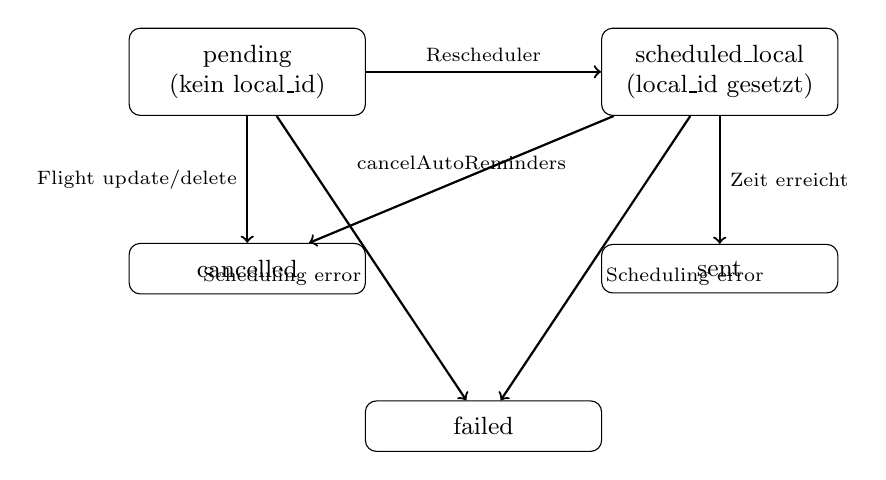
\begin{tikzpicture}[
    state/.style={draw, rounded corners, align=center, inner sep=6pt,
                  minimum width=3.0cm, font=\small},
    arr/.style={->, thick},
    lbl/.style={font=\scriptsize}
  ]
    \node[state] (pend)  at (0,0)     {pending\\(kein local\_id)};
    \node[state] (sched) at (6,0)     {scheduled\_local\\(local\_id gesetzt)};
    \node[state] (sent)  at (6,-2.5)  {sent};
    \node[state] (canc)  at (0,-2.5)  {cancelled};
    \node[state] (fail)  at (3,-4.5)  {failed};

    \draw[arr] (pend)  -- node[above,lbl]{Rescheduler} (sched);
    \draw[arr] (sched) -- node[right,lbl]{Zeit erreicht} (sent);
    \draw[arr] (pend)  -- node[left,lbl]{Flight update/delete} (canc);
    \draw[arr] (sched) -- node[above,lbl]{cancelAutoReminders} (canc);
    \draw[arr] (pend)  -- node[below left,lbl]{Scheduling error} (fail);
    \draw[arr] (sched) -- node[below right,lbl]{Scheduling error} (fail);
  \end{tikzpicture}
  \caption{Zustandsmodell der serverseitigen Notification-Registry}
  \label{fig:registry-state}
\end{figure}

Listing~\ref{lst:registry_insert} zeigt die vollständige Funktion zum Anlegen eines
Registry-Eintrags:

\begin{lstlisting}[style=skyline-ts,
  caption={Vollstaendiges registerNotification (services/notificationRegistry.ts)},
  label={lst:registry_insert}]
export async function registerNotification(
  userId: string,
  fireAt: string,
  kind: string,
  payload: Record<string, any>,
  localId?: string | null
): Promise<NotificationRecord | null> {
  try {
    const { data, error } = await supabase
      .from('notifications')
      .insert({
        user_id:  userId,
        fire_at:  fireAt,
        kind,
        payload,
        status:   'scheduled_local',
        local_id: localId ?? null,
      })
      .select()
      .single();
    if (error) throw error;
    return data as NotificationRecord;
  } catch (e) {
    if (__DEV__) console.warn('registerNotification failed', e);
    return null;
  }
}
\end{lstlisting}

Listing~\ref{lst:rescheduler} zeigt den vollständigen Rescheduler.
Auf iOS können lokale Notifications durch das Betriebssystem auch dann zugestellt werden,
wenn die App im Hintergrund oder vollständig beendet ist -- das iOS-eigene Scheduling
übernimmt die Auslieferung \cite{appleLocalNotif,expoNotificationsSDK}:

\begin{lstlisting}[style=skyline-ts,
  caption={Vollstaendiger reschedulePendingNotificationsForUser
           (services/notificationRescheduler.ts)},
  label={lst:rescheduler}]
export async function reschedulePendingNotificationsForUser(
  userId: string
): Promise<number> {
  try {
    const settings = await SettingsService.getInstance().getSettings();
    if (!settings.notifications) return 0;

    // Abgelaufene Eintraege als 'sent' markieren
    await cleanupPastNotifications(userId);

    // Offene Reminder ohne local_id aus Supabase holen
    const pending = await fetchPendingNotifications(userId);
    let scheduled = 0;

    for (const record of pending) {
      try {
        const payload = record.payload || {};
        const title   = payload.title || 'Reminder';
        const body    = payload.body  || '';
        const data    = payload.data  || {};

        const localId = await scheduleLocalNotificationId(
          title, body, record.fire_at, data
        );

        if (localId) {
          // local_id in Registry nachfuehren
          await updateNotificationLocalId(record.id, localId);
          scheduled++;
        } else {
          await markNotificationStatus(record.id, 'failed');
        }
      } catch (e) {
        if (__DEV__)
          console.warn('reschedule single notification failed', e);
        await markNotificationStatus(record.id, 'failed');
      }
    }
    return scheduled; // Anzahl erfolgreich neu eingeplanter Reminder
  } catch (e) {
    if (__DEV__)
      console.warn('reschedulePendingNotificationsForUser failed', e);
    return 0;
  }
}
\end{lstlisting}

% ============================================================
\subsection{Einstellungen, Quiet Hours und Testfunktionen}
\label{subsec:settings-quiet-hours}
% ============================================================

Die Konfiguration erfolgt über den Settings-Tab.
Die App bietet getrennte Toggles für Push Notifications allgemein, Boarding-,
Check-in-, Missing-Docs-, Receipt- sowie Note-/Checklist-Reminder, um Überlastung
und unnötige Unterbrechungen zu vermeiden
\cite{ozdemir2025echoes,visuri2019notifications}.
Quiet Hours verschieben geplante Notifications aus konfigurierten Ruhezeitfenstern
heraus (Listing~\ref{lst:quiet_hours}).

% Screenshot Settings
\begin{figure}[htbp]
  \centering
  \fbox{\parbox{0.88\textwidth}{\centering\vspace{1.2cm}
    \textbf{TODO: Screenshot einfügen}\\[0.3cm]
    App $\rightarrow$ Settings-Tab $\rightarrow$ Notifications-Sektion\\
    (Toggles für Reminder-Typen, Quiet-Hours-Konfiguration und
    ,,Send test notification''-Button)
    \vspace{1.2cm}}}
  \caption{Reminder-Einstellungen und Quiet-Hours-Konfiguration im Settings-Tab}
  \label{fig:settings_notif}
\end{figure}

Auf iOS erfordert das lokale Notification-System ausschließlich die Nutzer-Permission
(erteilt oder verweigert beim ersten Systemdialog) -- eine Channel-Konfiguration wie auf
Android entfällt \cite{appleLocalNotif,expoNotificationsSDK}.
Der Settings-Screen bietet eine ,,Send test notification''-Funktion,
die dieselben Scheduling-Helfer mit einem kurzen Offset von wenigen Sekunden verwendet
und die iOS-Permission sowie die Scheduling-Pipeline validiert.
Android-Channels sind im Code vorhanden, werden auf iOS ignoriert und wurden auf Android
nicht produktiv getestet \cite{androidNotifChannels}.

% ============================================================
\subsection{Pending-Notifications-Screen als Debug-Werkzeug}
\label{subsec:pending-screen}
% ============================================================

Zur Transparenz und Fehlersuche enthält Skyline einen Screen \emph{Pending notifications}.
Er kombiniert lokal geplante Notifications (via \texttt{getAllScheduledNotificationsAsync})
mit serverseitig offenen Registry-Einträgen (\texttt{fetchPendingNotifications})
\cite{expoNotificationsSDK}.
Listing~\ref{lst:pending_screen} zeigt das parallele Laden beider Datenquellen:

\begin{lstlisting}[style=skyline-ts,
  caption={Pending-Notifications-Screen: paralleles Laden lokaler und
           serverseitiger Daten (app/pending-notifications.tsx)},
  label={lst:pending_screen}]
// Beide Datenquellen parallel laden
const [localResult, serverResult] = await Promise.allSettled([
  // (a) lokal geplante Notifications vom OS-Scheduler
  Notifications.getAllScheduledNotificationsAsync(),
  // (b) offene Eintraege in der Supabase-Registry
  fetchPendingNotifications(userId),
]);

const localNotifs = localResult.status === 'fulfilled'
  ? localResult.value
  : [];
const serverNotifs = serverResult.status === 'fulfilled'
  ? serverResult.value
  : [];

// In der UI als kombinierte Liste dargestellt
// (Zeitpunkt, Titel, Body, Payload, Status)
setLocalItems(localNotifs);
setServerItems(serverNotifs);
\end{lstlisting}

% Screenshot Pending-Screen
\begin{figure}[htbp]
  \centering
  \fbox{\parbox{0.88\textwidth}{\centering\vspace{1.2cm}
    \textbf{TODO: Screenshot einfügen}\\[0.3cm]
    App $\rightarrow$ Pending-Notifications-Screen\\
    (Liste mit geplanten lokalen Notifications und Registry-Einträgen,
    inklusive Zeitpunkt, Status und Payload)
    \vspace{1.2cm}}}
  \caption{Pending-Notifications-Übersicht als Debug-Werkzeug in Skyline}
  \label{fig:pending_screen}
\end{figure}

% ============================================================
\section{Bewertung der Wirkung}
\label{sec:notifications-evaluation}
% ============================================================

Die Wirkung lässt sich entlang drei Dimensionen diskutieren:
Zuverlässigkeit, Effizienz und Nutzerakzeptanz.

\subsection{Zuverlässigkeit als KPI}

Ein zentraler KPI ist der Anteil der Flüge, bei denen keine kritischen Fehlzustände
auftreten (fehlende Unterlagen, versäumter Check-in).
Skyline erreicht Zuverlässigkeit durch:

\begin{itemize}
  \item korrekte Offset-Berechnung relativ zu \texttt{departureAt}/\texttt{arrivalAt}
        (Listing~\ref{lst:flight_offsets}),
  \item Cancel-/Reschedule-Mechanismus bei Flugupdates
        (Listing~\ref{lst:store_updateflight}),
  \item Quiet-Hours-Logik, die Notifications aus Ruhezeiten herausbewegt
        (Listing~\ref{lst:quiet_hours}),
  \item Registry als nachvollziehbare Quelle des Reminder-Zustands
        (Tabelle~\ref{tab:registry_status}).
\end{itemize}

\subsection{Effizienz als KPI}

Effizienz entsteht durch rechtzeitige Hinweise und Deep-Links in die konkrete Handlung.
Der Missing-Docs-Reminder (T$-$12\,h) gibt genug Zeit, fehlende Unterlagen hochzuladen;
der Receipt-Reminder (T$+$2\,h) unterstützt das zeitnahe Erfassen von Belegen nach Reisen
\cite{mitSavingReceipts}.
Deep-Links springen direkt in die Trip-Details mit offenem Dokumenten-Tab,
sodass der Weg von der Benachrichtigung zur konkreten Handlung minimal bleibt
\cite{reactNavDeepLink}.

\subsection{Nutzerakzeptanz}

Nutzerakzeptanz hängt stark davon ab, ob Erinnerungen als hilfreich oder störend
wahrgenommen werden.
Forschung zeigt, dass Notifications in unpassenden Kontexten als störend und
stressauslösend erlebt werden \cite{ozdemir2025echoes,visuri2019notifications}.
Skyline adressiert dies durch:

\begin{itemize}
  \item getrennte Toggles für jeden Reminder-Typ (granulare Kontrolle),
  \item konfigurierbare Quiet Hours (Listing~\ref{lst:quiet_hours}),
  \item Testfunktion zur risikofreien Validierung der Konfiguration.
\end{itemize}

% ============================================================
\section{Ergebnis}
\label{sec:notifications-result}
% ============================================================

Das Benachrichtigungs- und Erinnerungsmodul erhöht die Verlässlichkeit der
Reiseorganisation in Skyline, sofern die gewählten Offsets und Inhalte zum
Nutzungskontext passen.
Die Kombination aus zeitbasierten Offsets, Quiet Hours, Deep-Links und serverseitiger
Registry schafft einen erweiterbaren, nachvollziehbaren Reminder-Mechanismus
\cite{expoNotificationsSDK,supabaseSecuringApi,ozdemir2025echoes}.

\subsection{Reduktion kritischer Fehlzustände}
Durch gezielte Reminder für Check-in, Boarding und fehlende Unterlagen werden kritische
Fehlzustände reduziert.
Die Verbindung von Reminder-Text und Deep-Link minimiert den Weg zwischen Hinweis und
konkreter Handlung.

\subsection{Effizienzsteigerung}
Suchaufwand nach Unterlagen und der Nachbereitungsaufwand (Belege, Spesen) werden durch
das Modul gezielt reduziert -- ohne permanente Hintergrundprozesse oder serverseitige
Jobs, sondern durch lokales Scheduling und gezielte Trigger im Flight-Lifecycle.

\subsection{Gesamtbewertung}
Das Modul zeigt exemplarisch, wie ein theoretischer Ansatz (proaktive Systeme,
Notification Fatigue aus Kapitel~3) in eine konkrete, vollständig implementierte
Mobile-Funktion übersetzt werden kann.
Die Architektur ist ohne Umbau erweiterbar -- etwa durch APNs-basierte Server-Push-Flows
für iOS oder, zu einem späteren Zeitpunkt, durch eine vollständig getestete
Android-Unterstützung via FCM \cite{expoPushSetup,expoSendFcmApns}.
